%!TEX TS-program = xelatex
%!TEX encoding = UTF-8 Unicode
\documentclass[12pt, xcolor=dvipsnames]{beamer}
\definecolor{slight}{gray}{0.9}
\fboxsep=10pt
\usecolortheme[named=Royal Blue]{structure}
\useinnertheme{circles}
\usepackage[no-math]{fontspec}
\usepackage{xltxtra, xunicode}
\usepackage[utf8]{inputenc}
\usepackage{tikz}
%\usepackage[sc, osf]{mathpazo}
\usepackage[minionint, lf, mathtabular]{MinionPro}
\setmainfont[Mapping=tex-text]{Minion Web Pro}
\setsansfont[Mapping=tex-text]{Myriad Web Pro}
\setmonofont[Scale=MatchLowercase]{Source Code Pro}
\usefonttheme{professionalfonts}
%% 中文字配置
\usepackage[
CJKmath=true, indentfirst=false, PunctStyle={quanjiao},
CheckSingle=true, SlantFont, BoldFont
]{xeCJK}
\setCJKmainfont[Scale=0.9, BoldFont=Hiragino Mincho ProN W6]{Hiragino Mincho ProN W3}
%\setCJKmainfont[Scale=0.9, BoldFont=Noto Sans CJK JP Bold]{Noto Sans CJK JP Medium}
\setCJKsansfont[Scale=0.9, BoldFont=Hiragino Sans W6]{Hiragino Sans W4}
%\setCJKsansfont[Scale=0.9, BoldFont=Hiragino Sans CNS W6]{Hiragino Sans CNS W3}
%\setCJKsansfont[Scale=0.9, BoldFont=Hiragino Sans W7]{Hiragino Sans W4}
%\setCJKsansfont[Scale=0.9, BoldFont=Source Han Sans UI TC Bold]{Source Han Sans UI TC Regular}
%\setCJKsansfont[Scale=0.9, BoldFont=PingFang TC Semibold]{PingFang TC Regular}
\setCJKmonofont[Scale=0.9, BoldFont=Yuanti TC Regular]{Hiragino Maru Gothic ProN W4}
\usepackage{fancyvrb, attachfile2, pstricks}
\usepackage{graphicx}
\setbeamerfont{page number in head/foot}{size=\tiny}
\setbeamertemplate{footline}[frame number]
\usepackage{xmpmulti, booktabs, multicol}
\setbeamertemplate{navigation symbols}{}
\let\WriteBookmarks\relax
\usepackage{dcolumn}
\newcolumntype{.}[1]{D{.}{.}{#1}}
\newcolumntype{,}[1]{D{,}{,}{#1}}

\linespread{1.25}

\setbeamersize{text margin left=.8em, text margin right=.6em}

\makeatletter
\defbeamertemplate{itemize item}{mycircle}{\LARGE\raise-1.6pt\hbox{\textbullet}}
\makeatother

\setbeamertemplate{itemize item}[mycircle]
\setbeamertemplate{itemize subitem}[triangle]
\setlength\leftmargini{1.3em}
\setlength\leftmarginii{1em}


%\CTXFR
\title{\bf{\Huge {}\\[-2mm] Principles of Economics \\[2mm] Review Session}}
\author{{\Large 張耕齊\\[2mm] Keng-Chi Chang}}
\institute{{}\\[-7mm]\footnotesize\tt{<r03323070@ntu.edu.tw>}\\[2mm]}
\date{\large 2016.12.28}
\begin{document}
\fontsize{12}{14pt}\selectfont

\begin{frame}
\titlepage
\end{frame}





\begin{frame}
\frametitle{\bf §14.1 Market Structures}
\begin{center}
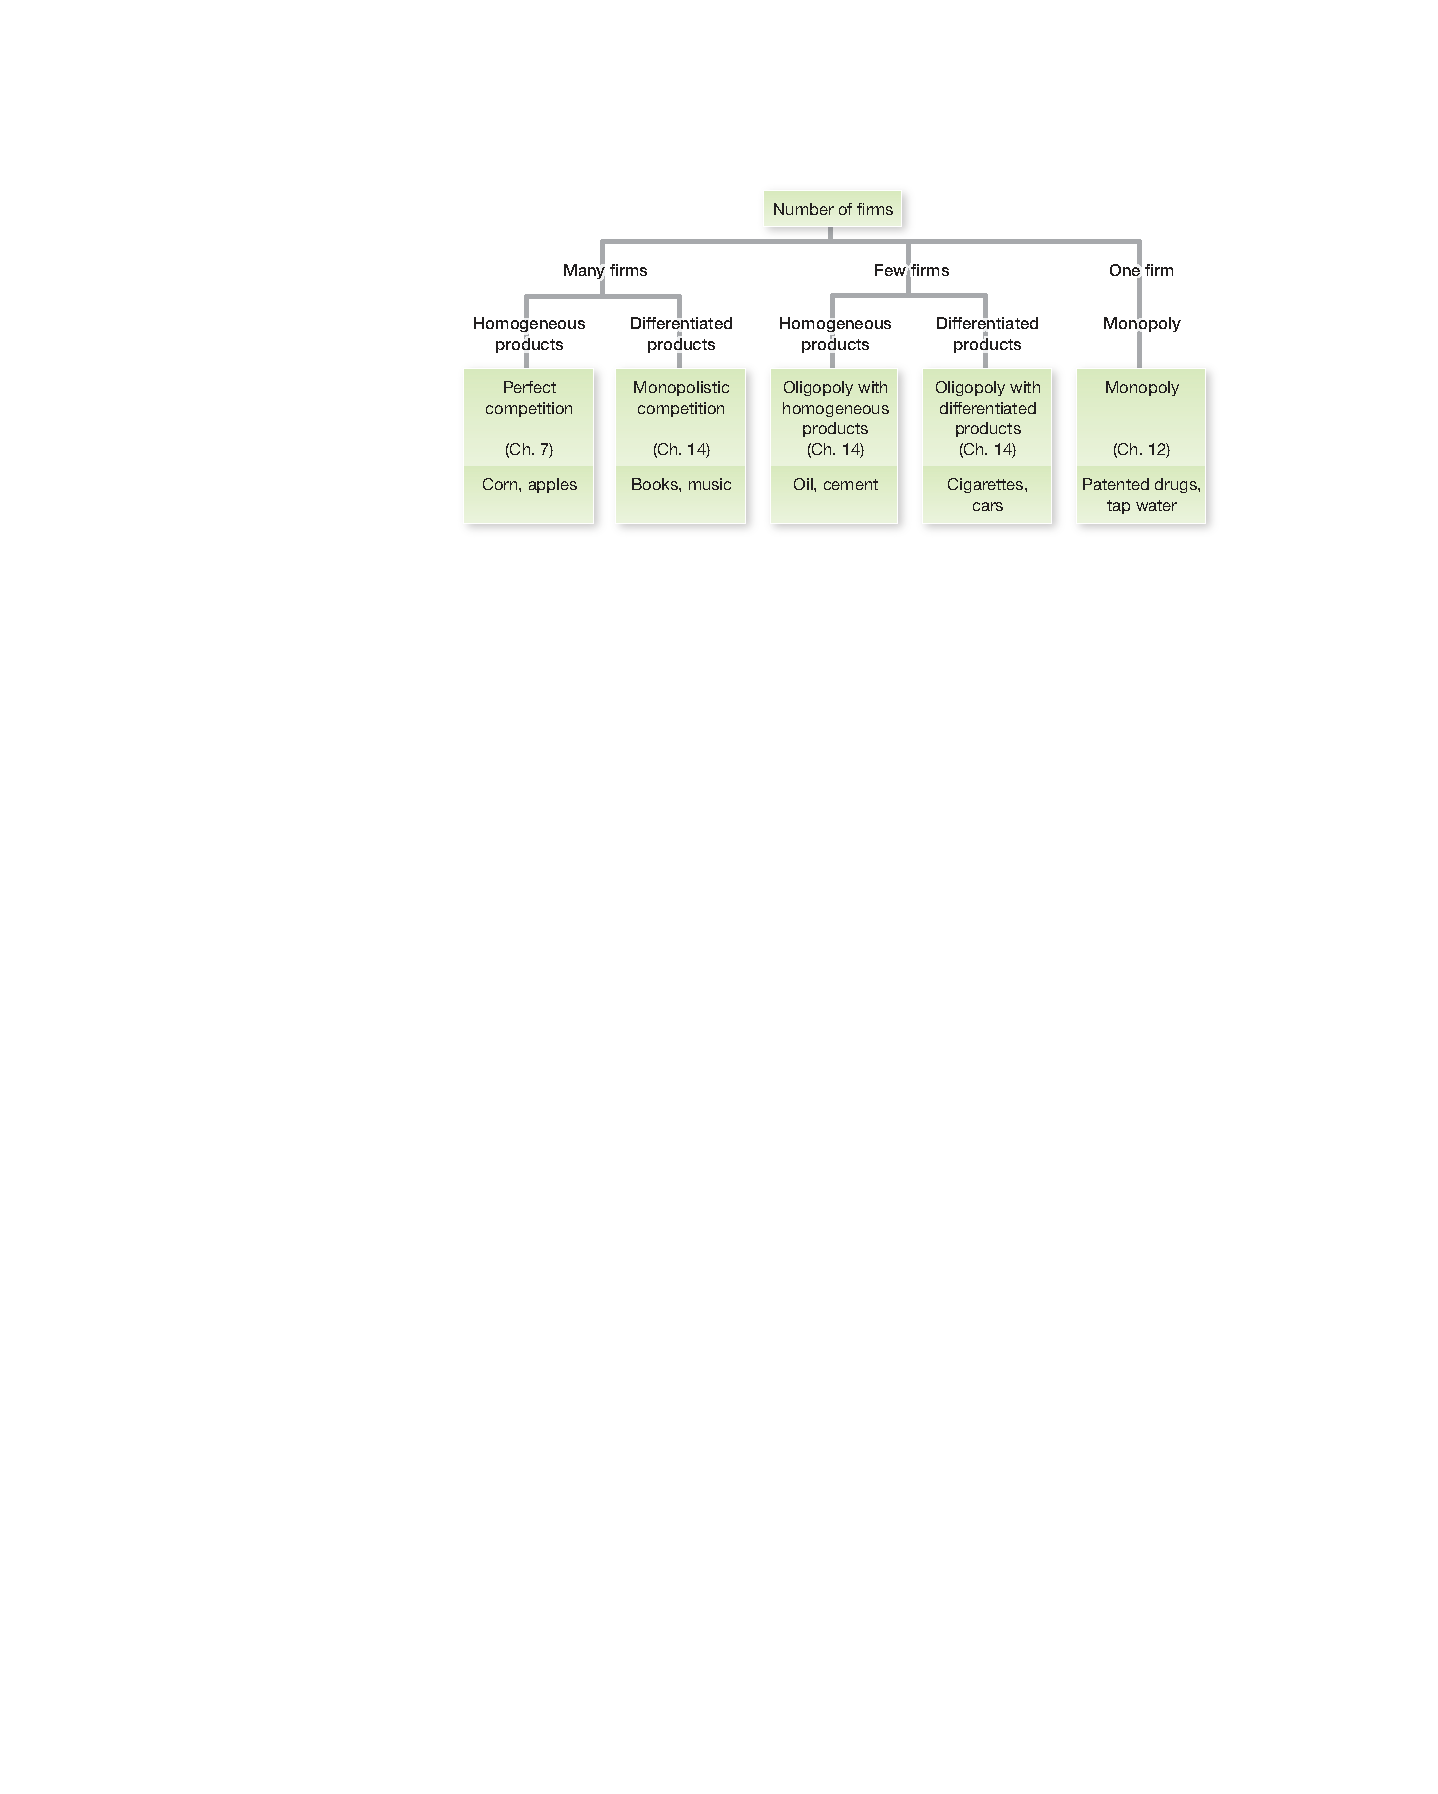
\includegraphics[width=\linewidth]{figures/14-1.pdf}
\end{center}
\end{frame}



\begin{frame}
\frametitle{\bf §14.2 Bertrand Duopoly 兩家廠商削價寡占}
\begin{itemize}
\item Homogenous goods in the market
\item Bertrand: simultaneous choose price; Duopoly: 2 firms
\item Like a simultaneous move game
\begin{itemize}
\item Firms set a price (best response) depending on the guess of the other's price
\item Obtain a Nash equilibrium if both firms are best responding each other
\end{itemize}
\item Often this is enough to generate an outcome close to perfect competition (see the textbook example)
\item You may learn other forms of oligopoly in the future
\end{itemize}
\end{frame}


\begin{frame}
\frametitle{\bf §14.2 Collusion 勾結 / Cartel 聯合壟斷}
\begin{itemize}
\item Firms may have incentive to cooperate with each other and act like a monopolist and earn a high share of profit
\item But this is difficult to maintain, since this is usually not their best response, they will have an incentive to cheat on each other, so this will break the monopoly-like outcome
\item Consider the previous textbook example, if they collude, ...
\end{itemize}
\end{frame}



\begin{frame}
\frametitle{\bf Homogenous Oligopoly and Collusion}
\small \textsf{\bfseries ALL 14-10.} Suppose the world demand schedule for oil is as follows. There are two oil-producing countries, A and B. Each will produce either 10 or 20 barrels of oil. To keep things simple, assume they can produce this oil at zero cost.
\begin{center}
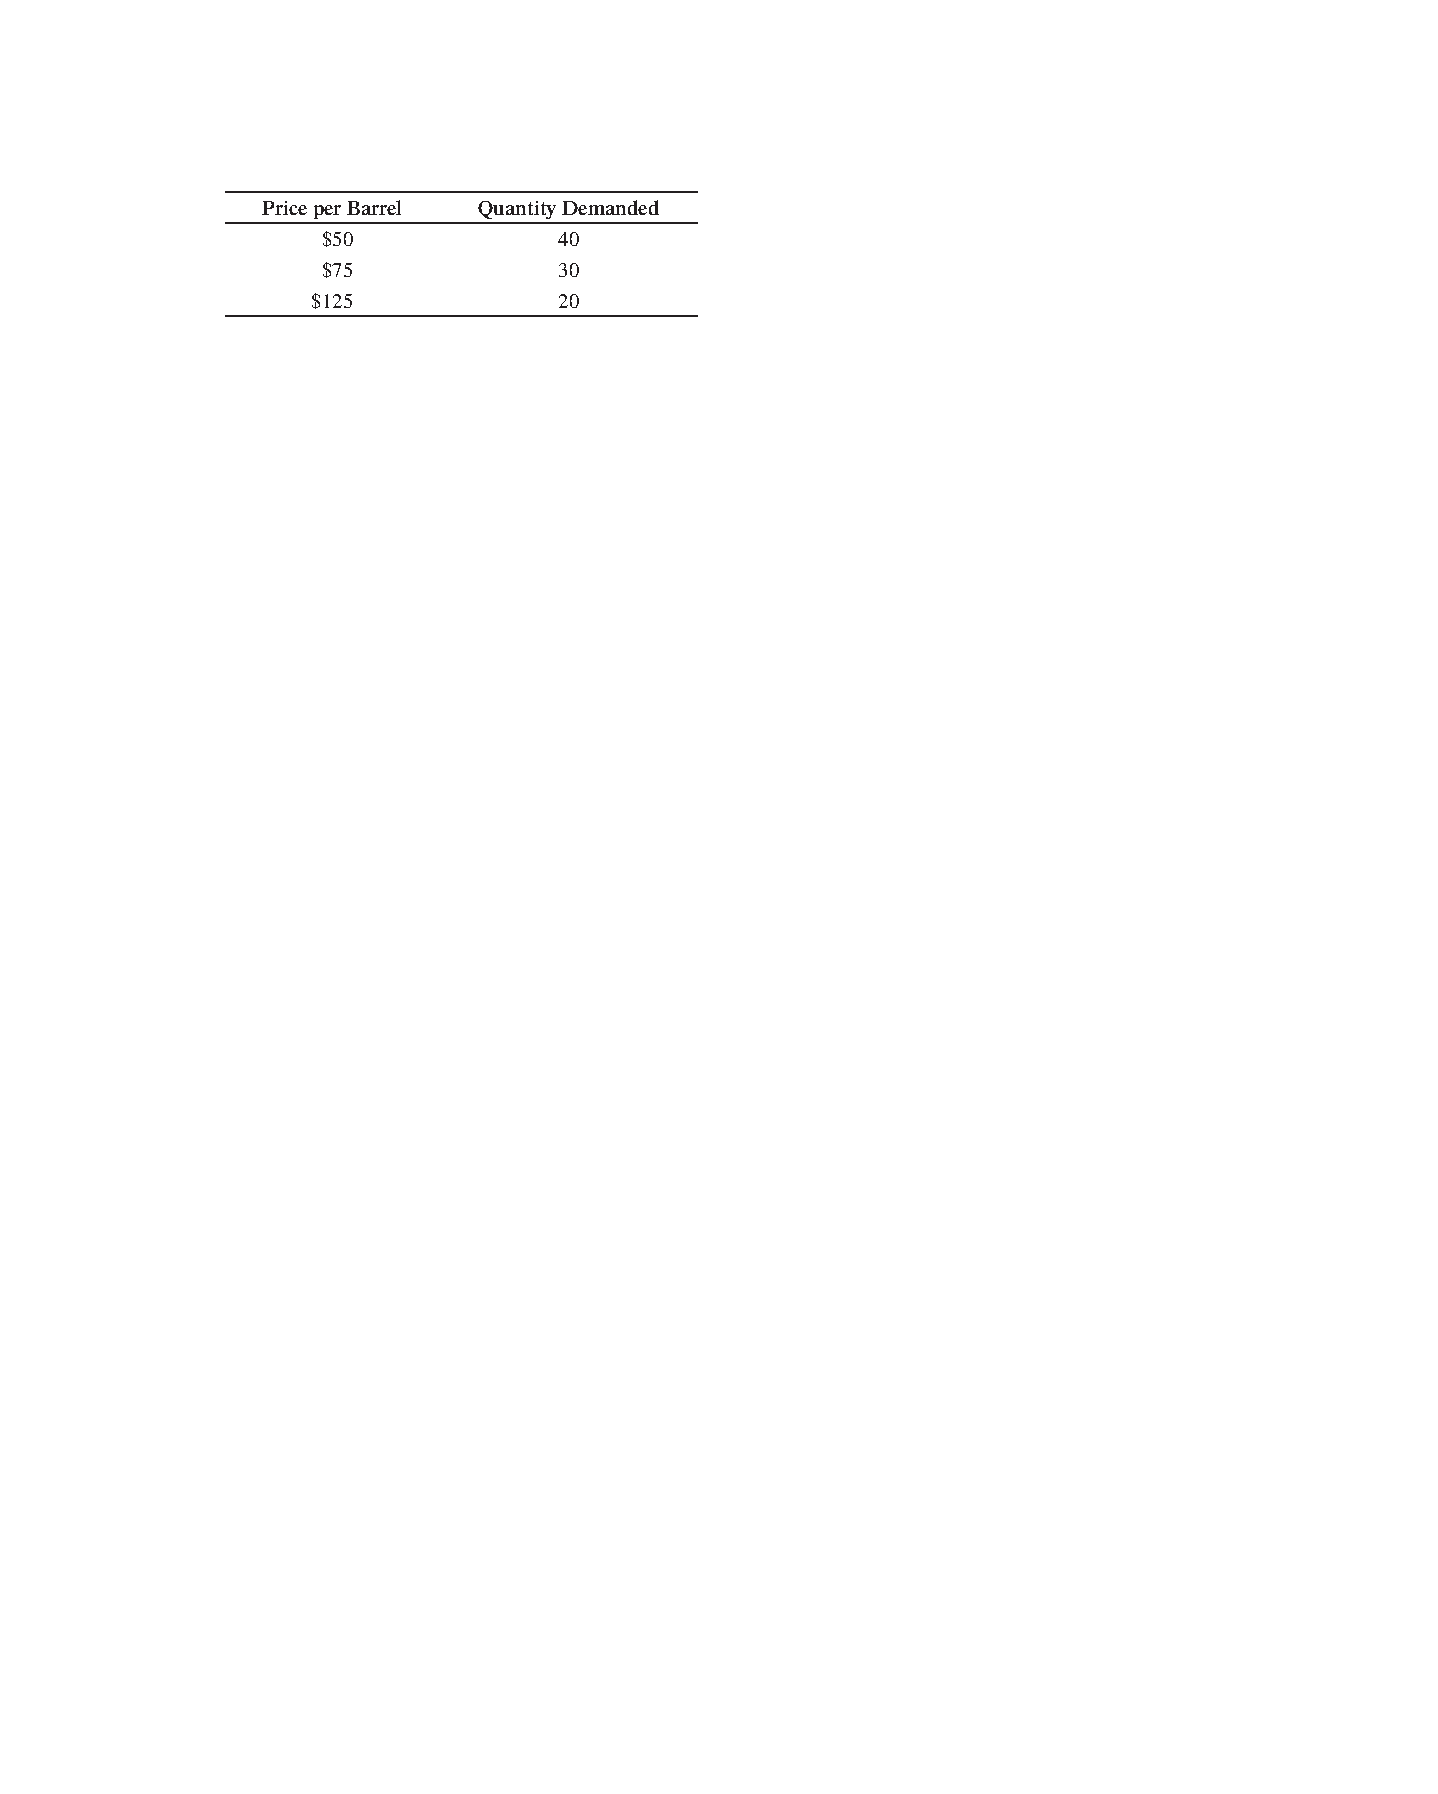
\includegraphics[width=.6\linewidth]{figures/p10.pdf}
\end{center}
\end{frame}


\begin{frame}
\small 
\begin{enumerate}\itemsep-0.5ex 
\item[a.] There are four possible outcomes: A produces 10 or 20 and B produces 10 or 20. Find each country’s profit for each of these four possibilities.
\item[b.] Suppose these countries choose the quantity of oil to produce simultaneously and without consulting with one another. Show that each country will produce 20 barrels of oil and each will earn a profit of \$1,000.
\item[c.] The oil ministers realize they can do better if they collude and agree that each will produce 10. How much profit will each country earn if each produces 10 instead of 20?
\item[d.] Will country A have an incentive to cheat and produce 20 instead of 10? Will country B have an incentive to cheat and produce 20 instead of 10?
\end{enumerate}
\end{frame}


\begin{frame}
\frametitle{\bf §14.3 Monopolistic Competition 獨占性競爭}
\begin{itemize}
\item Monopolistic competition and oligopoly with differentiated products are very similar, other than the former has many sellers and the latter has only a few
\item They are also very similar to what you have learned in monopoly
\item In monopoly, there is only one seller and hence one product, the firm must face the whole downward-sloping demand curve
\item In monopolistic competition and oligopoly with differentiated products, since there are different kinds of goods, the demand curve a single firm faces (or the so-called {\it residual demand}) is also downward-sloping, and hence so does $MR$
\item In contrast, under perfect competition, a single firm faces a horizontal demand curve since they are price takers, so does $MR$
\end{itemize}
\end{frame}



\begin{frame}
\frametitle{\bf Profit under Monopolistic Competition}
\begin{center}
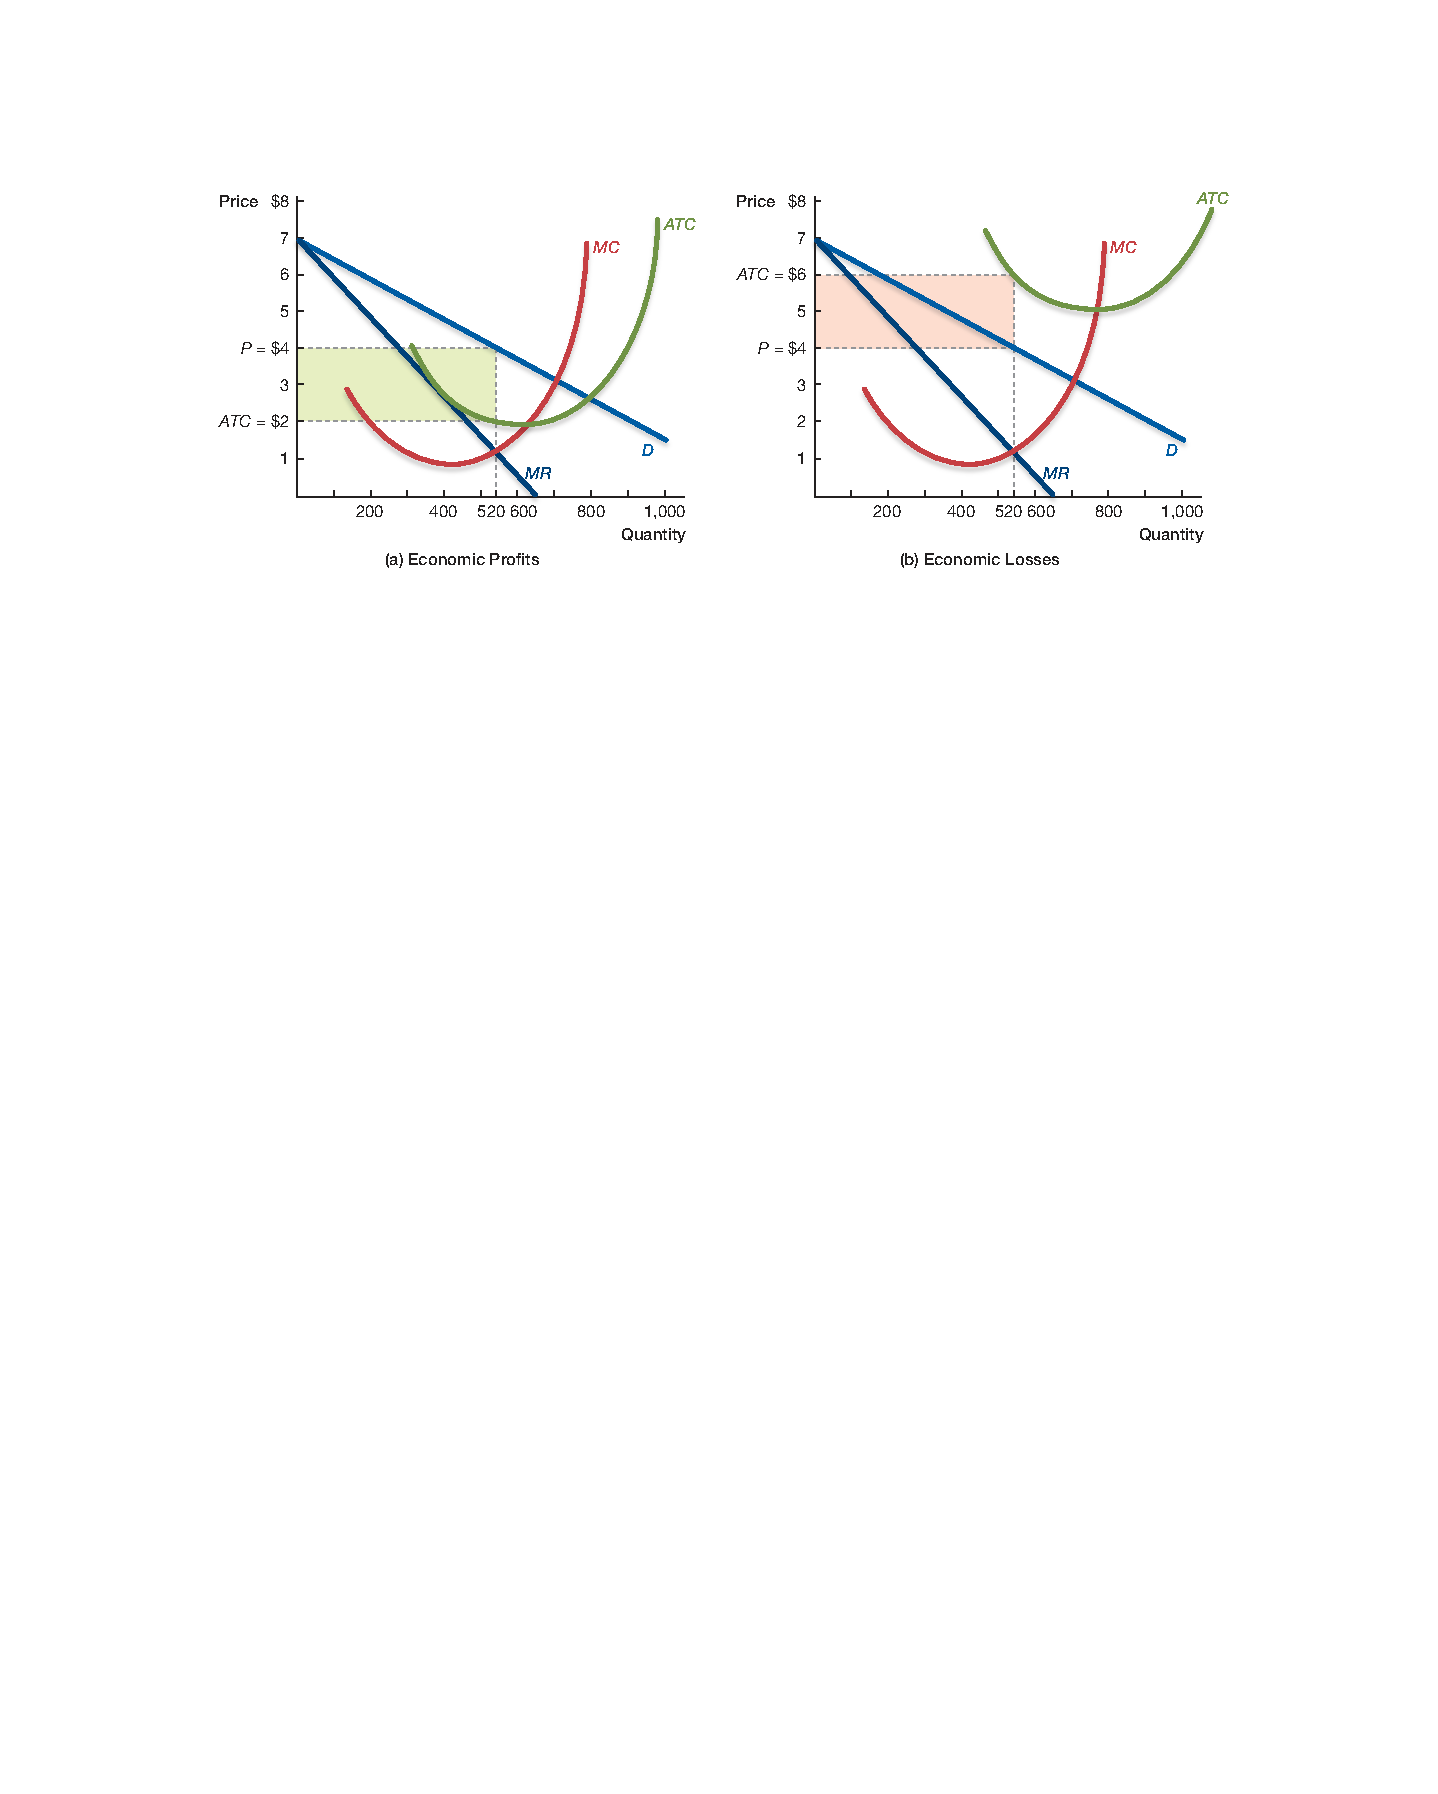
\includegraphics[width=\linewidth]{figures/14-7.pdf}
\end{center}
\end{frame}





\begin{frame}
\frametitle{\bf Monopolistic Competition is Inefficient}
\begin{center}
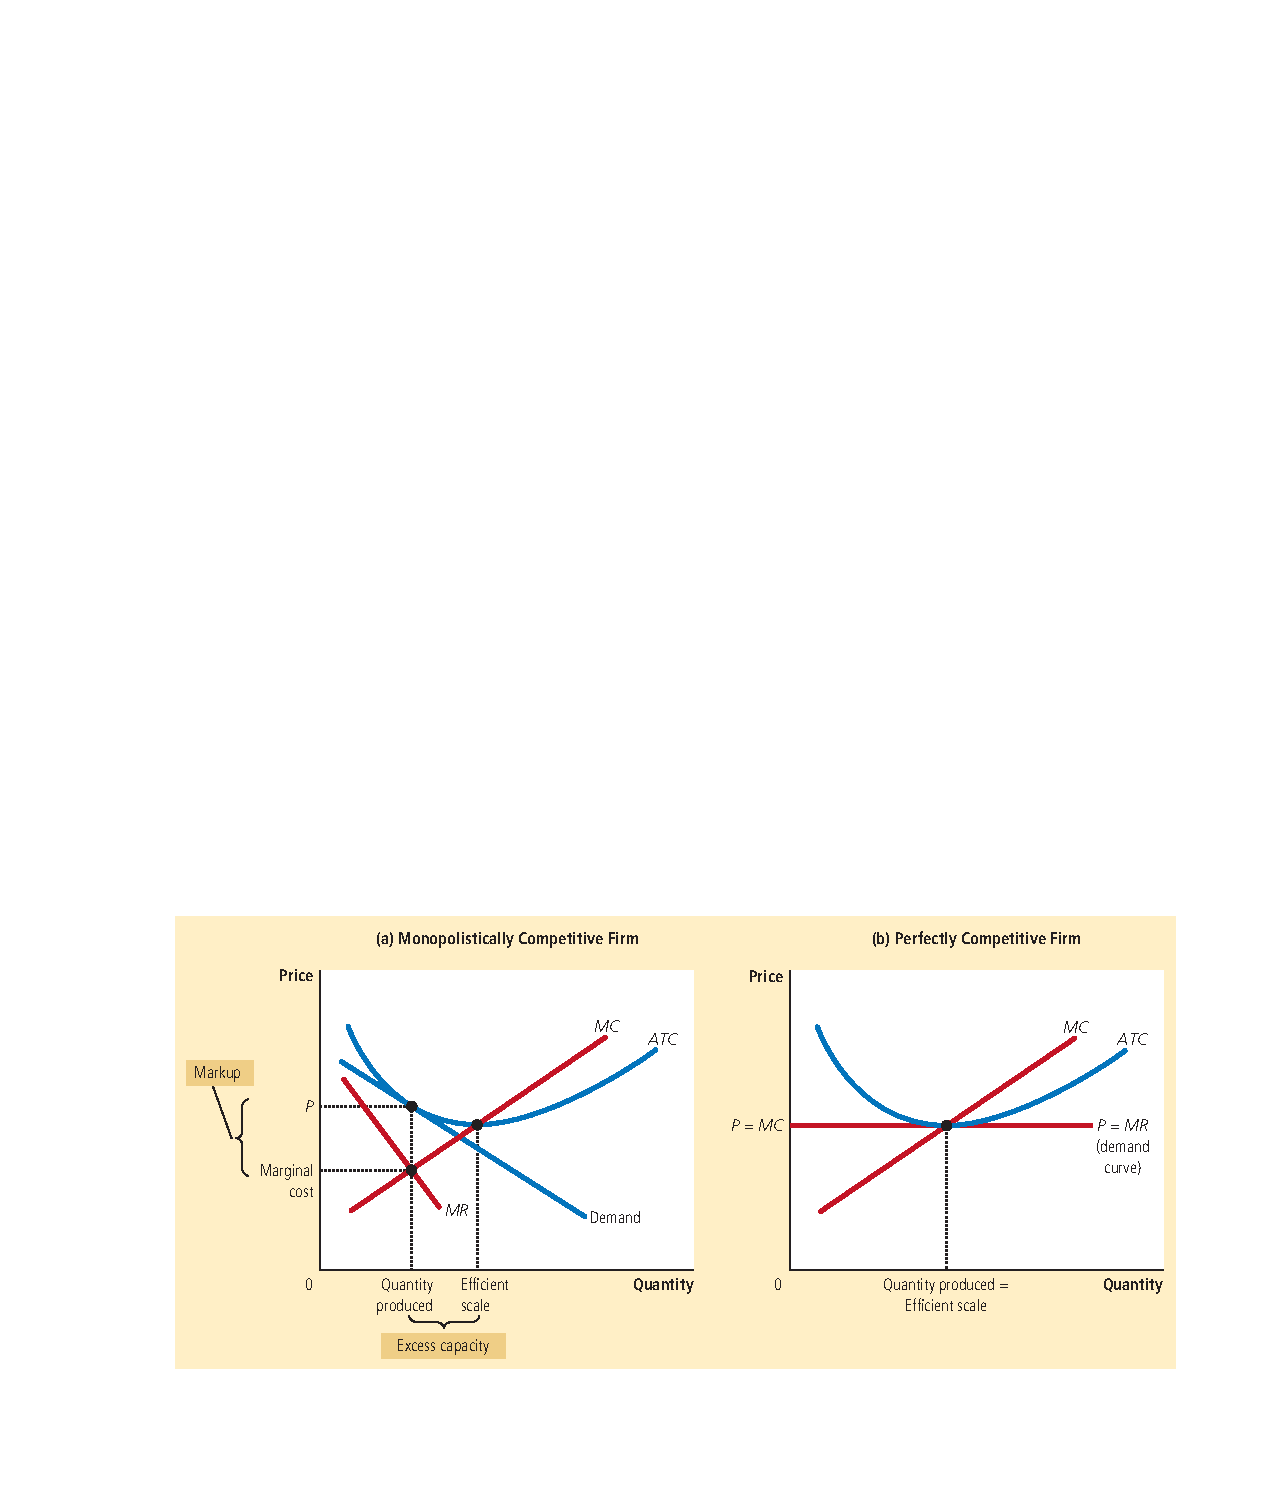
\includegraphics[width=\linewidth]{figures/14-10.pdf}
\end{center}
\end{frame}





\begin{frame}
\frametitle{\bf Near Perfect Competition}
\small \textsf{\bfseries Final 2011 Essay B.} \\
(omitted) Mr. Liu's livelihood is now just as precariously balanced. He reckons his cooking-oil costs shot up 27\% in 2010... (omitted)\\
In recent weeks, Beijing has moved to snuff out rumors that cooking oil is in short supply by auctioning millions of metric tons from strategic national reserves in Xinjiang and Shandong. The national planning agency has declared that supply 'is completely guaranteed.' In November, China's government ordered the largest producers to cap their retail prices through March. And it quintupled the fine for conspiring to raise prices to 5 million yuan, or \$750,000.
\end{frame}





\begin{frame}
\small 
For now, the measures appear to have put a lid on edible-oil prices. Yet one midsize producer in Shanghai says they are also discouraging production. The company's general manager, who asked not to be identified, said he would normally be maximizing output ahead of the Lunar New Year in early February but has deactivated half his plant. (omitted)\\
Cooking oil is a rising concern of food vendor Mr. Liu and his wife, whose \$105 daily sales from their tiny Shanghai stall go to support their two children who live back in their home province of Shandong. Despite the higher price for soybean oil, Mr. Liu shudders at the risk he faces in lifting his 10.5-cent charge for a flaky sweet bun. `Customers would disappear,' he says.
\end{frame}





\begin{frame}
\small 
\begin{enumerate}\itemsep-0.5ex 
\item[2.] Draw a graph to illustrate the demand curve and marginal revenue curve Mr. Liu’s breakfast stand is facing.
\item[5.] What is the reaction of the government to this price surge? Do you think its regulatory measures are effective? Why or why not?
\end{enumerate}
\end{frame}





\begin{frame}
\frametitle{\bf Monopsony 獨買}
\small \textsf{\bfseries Final 2010 Essay B.} \\
\begin{enumerate}\itemsep-0.5ex 
\item[1.] Consider the labor market for Nan Shan Life Insurance employees after the merger, in which the take-over firm, Chinatrust Financial Holdings, is the monopsony (single buyer), and former Nan Shan Life Insurance employees are the only group of sellers. How does Chinatrust determine its ``demand'' for Nan Shan employees?
\item[2.] Draw a diagram and find Chinatrust’s profit maximizing wage and quantity. (Hint: This is the ``reverse'' of a monopoly, with a ``supply curve + marginal cost curve'' instead of a ``demand curve + marginal revenue curve.'')
\item[3.] Is the monopsony outcome efficient? Why or why not?
\end{enumerate}
\end{frame}





\end{document}